\section{动态规划Professional------树形DP、状压DP与数位DP}
这一部分让我们看看\sout{非常水的}丧心病狂的DP类型,在NOIp 2017中首次出现了以前只出现在省选等高水平比赛中的DP类型------状压DP,这种类型的DP本质上是枚举状态(和搜索一样),但是又具有DP的某些特性。所以比较困难。树形DP则是另外一种不是很常见的DP类型,就是将DP的位置由矩阵上转移到树上来做。最后是最少见的数位DP。\sout{其实也不是非常难。}
\subsection{树形DP}
\begin{definition}[树形DP]就是把普通的DP转移到树上来做,转移方向就是由普通的在数组转移变为在树上借助边转移。其他的内容与普通DP无异。唯一需要注意的是\textcolor{red}{\textbf{先DP儿子节点}}。
\end{definition}

以上是对树形DP的定义,可以看出来它与普通的DP没什么区别。

为什么要先对儿子进行DP呢?其实非常简单,树的结构是由下而上越来越小的,如果先DP父亲节点,那么由于儿子节点还没有被更新,仍然保持初始值0,自然无法更新父亲节点。所以要先对较小规模的问题求解,即先处理依赖关系较少的节点(状态转移的基本性质,未知量由已知量转移而来)。

下面通过一道题目来说明一下树形DP的基本过程。
\begin{example}选课\\
	\textbf{题目描述}

	在大学里每个学生,为了达到一定的学分,必须从很多课程里选择一些课程来学习,在课程里有些课程必须在某些课程之前学习,如高等数学总是在其它课程之前学习。现在有N门功课,每门课有个学分,每门课有一门或没有直接先修课(若课程a是课程b的先修课即只有学完了课程a,才能学习课程b)。一个学生要从这些课程里选择M门课程学习,问他能获得的最大学分是多少?
	\ \\
	\textbf{输入输出格式}
	\ \\
	\textbf{输入格式:}

	第一行有两个整数N,M用空格隔开。(1<=N<=300,1<=M<=300)

	接下来的N行,第I+1行包含两个整数ki和si, ki表示第I门课的直接先修课,si表示第I门课的学分。若ki=0表示没有直接先修课(1<=ki<=N, 1<=si<=20)。
	\\
	\textbf{输出格式:}

	只有一行,选M门课程的最大得分。
	\\
	\textbf{输入输出样例}
	\\
	\textbf{输入样例:}
	\begin{minted}{text}
7  4
2  2
0  1
0  4
2  1
7  1
7  6
2  2
\end{minted}
	\textbf{输出样例:}
	\begin{minted}{text}
13
\end{minted}
\end{example}

题目大意是给定一个有依赖关系的课程安排表,一个课程可能依赖于多个课程,也可能被多个课程依赖,每学一个课程都能获得一些学分,最多学习M个课程,求能获得最大学分。

很明显,这是一个DAG(有向无环图),也就是一棵树。依赖关系可能不连续,也就是说给定的是一个森林。

对于森林的问题,我们可以通过虚拟一个总根节点,森林中所有的根节点都向这个总根节点连一条无向边,然后这个虚拟节点上的答案就是问题的答案。

因为树形数据结构是递归定义的(父亲节点与儿子节点,递归起点可以看做是根节点或某一个叶子节点,都可以遍历完整棵树),所以树形DP的基本思路应该是对树的每一个节点递推地计算该点的最优解,需要使用到DFS。

这道题的状态转移方程不难想到,设状态$f[i][j]$表示第i个节点取j个子节点(不包括自己)所取得的最大(最小)收益。然后标准状态转移模板就是$f[i][j]=\max(f[i][j],f[i][j-k]+f[儿子节点编号][k])$

现在考虑一下一棵子树的根节点可能会有多个儿子的情况。传统上有两种解决方案,第一种就是直接DFS,DP需要用到子树的时候就DFS这棵子树,不去考虑儿子的个数的问题。

这种做法的代码如下:
\begin{minted}{C++}
#include <cstdio>
#include <cstring>
#include <algorithm>
using namespace std;
int n,m,f[2005][2005];
int head[2005],next[2005],w[2005];
int dfs(int x){
    if (head[x]==-1) return 0;
    int sum=0;
    for (int i=head[x];i!=-1;i=next[i])
    {
        int t=dfs(i);
        sum+=t+1;
        for (int j=sum;j>=0;j--)
        {
            for (int k=0;k<=t;k++)
                if (j-k-1>=0) f[x][j]=max(f[x][j],f[x][j-k-1]+f[i][k]);
        }
    }
    return sum;
}
int main()
{
    scanf("%d%d",&n,&m);
    memset(f,0,sizeof(f));
    memset(head,-1,sizeof(head));
    for (int i=1;i<=n;i++)
    {
        int a;
        scanf("%d%d",&a,&w[i]);
        next[i]=head[a];
        head[a]=i;
    }
    for (int i=1;i<=n;i++) f[i][0]=w[i];
    f[0][0]=0;
    dfs(0);
    printf("%d",f[0][m]);
    return 0;
\end{minted}

另外一种做法是多叉树转为二叉树来做。多叉树转二叉树在树这一节内容lpy学姐已经给你们讲过了,就是左儿子右兄弟表示法,我就不讲了,直接说思路。

用f[root][k]表示第root节课为根且还剩k个自由选课数时,学分的最大值;
\begin{itemize}
	\item{不选此课,它与它的后续值皆为零;}
	\item{选此课,最终求max【它的值+兄弟与左孩子瓜分剩余选课数时最优解,原状态,不选它(但它兄弟的状态要与它合并,因为左孩子只有一个)】}
\end{itemize}

树形DP本质上是对这棵树的DFS操作。需要写个记忆化搜索优化一下。

于是就可以写出代码:

\begin{minted}{C++}
#include<cstdio>
#include<cstring>
using namespace std;
const int N=320;
int n,m;
int f[N][N],b[N],c[N],s[N];
void dp(int root,int k)
{
    if(f[root][k]>=0)return;
    if(root==0||k==0){f[root][k]=0;return;}
    dp(b[root],k);//兄弟与左孩子享有同等权利;
    for(int i=0;i<k;i++)
    {
        dp(c[root],k-i-1);//选第root门课; 
        dp(b[root],i);// 因为根节点给下一代指标时,只会给左孩子,所以下一代的左孩子要分给兄弟指标;
        f[root][k]=max(f[root][k], max(f[b[root]][k], f[b[root]][i] + f[c[root]][k - i - 1] + s[root]));
        //求三个状态最大值:选此状态(原封不动),不选,选此状态(更新,此节点+瓜分指标后的兄弟与左孩子的最优解) 
    }
}
int main()
{
    cin>>n>>m;
    int fa;
    for(int i=1;i<=n;i++)
    {
        cin>>fa>>s[i];
        if(fa==0)fa=n+1; 
        b[i]=c[fa];//c[i]记录的是长子,长子把‘长子’的位子让给i,原长子成为了新长子兄弟, 
        c[fa]=i;//父亲直辖原长子; 
    }
    memset(f,-1,sizeof(f));
    dp(c[n+1],m);
    cout<<f[c[n+1]][m];//无先修课的的最优值会集中于c[n+1]; 
    return 0;
}
\end{minted}
\begin{center}
\includegraphics[scale=1.75]{64304330_p0.png}\end{center}
\note
\subsection{状压DP}
\subsubsection{定义与特点}
\begin{definition}[状压DP]和普通的DP一样,同样需要设计状态与状态转移方程,保存一些状态来相互转移的解题过程,与普通DP不同的是,状压DP的状态不是简单的状态,而是\textbf{不同的方案}等等。状态压缩中的状态常用二进制来表示,转移过程常用位运算来完成。
\end{definition}

以上是我给状压DP的简单定义。或许不是非常准确,但是基本能反映出状压DP的含义了。如果不是特别理解的话,还是联想DP最初的定义,就是一个无限优化的搜索。只不过这个优化有点特殊,表示的状态与常见的DP有些不同。

状压DP的特点:\textcolor{red}{\textbf{数据范围非常小,一般有$n\leq 24$}},因为状压DP需要枚举每一个子集。

学习状压DP前首先需要了解位运算的相关知识。让我们先来看一下。
\subsubsection{有关位运算的知识}
设有一个集合$S$,用一个二进制数表示集合中每一个元素的选择情况(第$i$个二进制位为0表示不选集合$S$中的第$i$个元素,当然这个集合不具有数学上集合的无序性,要求是按编号有序排列的),则这个二进制数表示的是集合$S$的一个子集。

状压DP就是枚举子集,转移常常涉及对并集,交集、补集的操作。可以使用位运算来进行加速对集合的运算。

设有两个集合$S_1\subset S, S_2\subset S$,则我们有以下集合运算与位运算的关系:

\begin{center}
	\begin{tabular}{|c|c|}
		\hline
		集合运算               & 与之等价的位运算                   \\
		\hline
		$S_1\cap S_2$          & $S_1$ \verb+&+ $S_2$ \\
		\hline
		$S_1\cup S_2$          & $S_1$ \verb+|+ $S_2$ \\
		\hline
		$\complement_{S_1}S_2$ & $S_1$ \verb+^+ $S_2$ \\
		\hline
	\end{tabular}
\end{center}

状压的一些技巧:
\begin{itemize}
	\item{若S是U的子集,则S关于U的补集为:\verb$S^U$}
	\item{判断点$k$是否在集合S中(即S的第$k- 1$位是否为1):\\\verb$S&(1<<(k-1))!=0?"Yes":"No";$}
	\item{枚举S的子集:\verb$for(int i=S;i;i=(i-1)&S){...}$}
	\item{设置一个大小为n的全集:\verb$n=1<<(n-1)$}
\end{itemize}

下面给出两道例题,再细致地谈一下状压DP的内容和实现细节。

\subsubsection{基础例题---愤怒的小鸟}
\begin{example}愤怒的小鸟\\
\textbf{问题描述}

Kiana最近沉迷于一款神奇的游戏无法自拔。

简单来说,这款游戏是在一个平面上进行的。

有一架弹弓位于$(0,0)$处,每次Kiana可以用它向第一象限发射一只红色的小鸟,小鸟们的飞行轨迹均为形如$y=ax^2+bx$的曲线,其中a,b是Kiana指定的参数,且必须满足$a\leq 0$。

当小鸟落回地面(即x轴)时,它就会瞬间消失。

在游戏的某个关卡里,平面的第一象限中有n只绿色的小猪,其中第i只小猪所在的坐标为$(xi,yi)$。

如果某只小鸟的飞行轨迹经过了$(xi,yi)$,那么第i只小猪就会被消灭掉,同时小鸟将会沿着原先的轨迹继续飞行;

如果一只小鸟的飞行轨迹没有经过$(xi,yi)$,那么这只小鸟飞行的全过程就不会对第i只小猪产生任何影响。

例如,若两只小猪分别位于$(1,3)$和$(3,3)$,Kiana可以选择发射一只飞行轨迹为$y=-x^2+4x$的小鸟,这样两只小猪就会被这只小鸟一起消灭。

而这个游戏的目的,就是通过发射小鸟消灭所有的小猪。

这款神奇游戏的每个关卡对Kiana来说都很难,所以Kiana还输入了一些神秘的指令,使得自己能更轻松地完成这个游戏。这些指令将在【输入格式】中详述。

假设这款游戏一共有T个关卡,现在Kiana想知道,对于每一个关卡,至少需要发射多少只小鸟才能消灭所有的小猪。由于她不会算,所以希望由你告诉她。

\textbf【输入格式】

第一行包含一个正整数T,表示游戏的关卡总数。

下面依次输入这T个关卡的信息。每个关卡第一行包含两个非负整数n,m,分别表示该关卡中的小猪数量和Kiana输入的神秘指令类型。接下来的n行中,第i行包含两个正实数(xi,yi),表示第i只小猪坐标为(xi,yi)。数据保证同一个关卡中不存在两只坐标完全相同的小猪。

如果m=0,表示Kiana输入了一个没有任何作用的指令。

如果m=1,则这个关卡将会满足:至多用$\left \lceil \frac{n}{3} + 1 \right \rceil$只小鸟即可消灭所有小猪。

如果m=2,则这个关卡将会满足:一定存在一种最优解,其中有一只小鸟消灭了至少$\left \lfloor \frac{n}{3} \right \rfloor$只小猪。

保证$1\leq n\leq 18,0\leq m\leq 2,0\leq x_i,y_i\leq 10$,输入中的实数均保留到小数点后两位。

上文中,符号$\left \lceil x \right \rceil$和$\left \lfloor x \right \rfloor$分别表示对c向上取整和向下取整。\\
\textbf{【输出格式】}

对每个关卡依次输出一行答案。

输出的每一行包含一个正整数,表示相应的关卡中,消灭所有小猪最少需要的小鸟数量。\\
\textbf{【输入样例$1$】}
\begin{minted}{text}
2
2 0
1.00 3.00
3.00 3.00
5 2
1.00 5.00
2.00 8.00
3.00 9.00
4.00 8.00
5.00 5.00
\end{minted}
\textbf{【输出样例$1$】}
\begin{minted}{text}
1
1
\end{minted}
\textbf{【输入样例$2$】}
\begin{minted}{text}
3
2 0
1.41 2.00
1.73 3.00
3 0
1.11 1.41
2.34 1.79
2.98 1.49
5 0
2.72 2.72
2.72 3.14
3.14 2.72
3.14 3.14
5.00 5.00
\end{minted}
\textbf{【输出样例$2$】}
\begin{minted}{text}
2
2
3
\end{minted}
\textbf{【输入样例$3$】}
\begin{minted}{text}
1
10 0
7.16 6.28
2.02 0.38
8.33 7.78
7.68 2.09
7.46 7.86
5.77 7.44
8.24 6.72
4.42 5.11
5.42 7.79
8.15 4.99
\end{minted}
\textbf{输出样例$3$}
\begin{minted}{text}
6
\end{minted}
\textbf{【说明】}\\
\textbf{【样例解释1】}

这组数据中一共有两个关卡。

第一个关卡与【问题描述】中的情形相同,2只小猪分别位于$(1.00,3.00)$和$(3.00,3.00)$,只需发射一只飞行轨迹为$y = -x^2 + 4x$的小鸟即可消灭它们。

第二个关卡中有$5$只小猪,但经过观察我们可以发现它们的坐标都在抛物线 $y = -x^2 + 6x$上,故Kiana只需要发射一只小鸟即可消灭所有小猪。
\ \\
\textbf{【数据范围】}
\begin{center}
\begin{tabular}{c|c|c|c}
\Xhline{1.2pt}
测试点编号&$n$&$m$&$t$\\
\Xhline{1.2pt}
$1$&\multirow{2}{*}{$\leq 2$}&\multirow{12}{*}{$=0$}&$\leq 10$\\
\cline{1-1}\cline{4-4}
$2$&&&$\leq 30$\\
\cline{1-2}\cline{4-4}
$3$&\mr{2}{$\leq 3$}&&$\leq 30$\\
\cline{1-1}\cline{4-4}
$4$&&&$\leq 30$\\
\cline{1-2}\cline{4-4}
$5$&\mr{2}{$\leq 4$}&&$\leq 10$\\
\cline{1-1}\cline{4-4}
$6$&&&$\leq 30$\\
\cline{1-2}\cline{4-4}
$7$&$\leq 5$&&\mr{4}{$\leq 10$}\\
\cline{1-2}
$8$&$\leq 6$&&\\
\cline{1-2}
$9$&$\leq 7$&&\\
\cline{1-2}
$10$&$\leq 8$&&\\
\cline{1-2}\cline{4-4}
$11$&$\leq 9$&&\mr{4}{$\leq 30$}\\
\cline{1-2}
$12$&$\leq 10$&&\\
\cline{1-3}
$13$&\mr{2}{$\leq 12$}&$=1$&\\
\cline{1-1}\cline{3-3}
$14$&&$=2$&\\
\cline{1-4}
$15$&\mr{3}{$\leq 15$}&$=0$&\mr{3}{$\leq 15$}\\
\cline{1-1}\cline{3-3}
$16$&&$=1$&\\
\cline{1-1}\cline{3-3}
$17$&&$=2$&\\
\cline{1-4}
$18$&\mr{3}{$\leq 18$}&$=0$&\mr{3}{$\leq 5$}\\
\cline{1-1}\cline{3-3}
$19$&&$=1$&\\
\cline{1-1}\cline{3-3}
$20$&&$=2$&\\
\Xhline{1.2pt}
\end{tabular}
\end{center}
\end{example}

考虑一下,有思路吗?

其实这个数据范围,暴力也可以过。大家不妨先写个暴力玩玩。

因为状态的数目不是很多,所以我们考虑用二进制数来表示抛物线打掉的猪的集合。用0和1表示是否选中这一只猪,若二进制的第$i$位为表示选第$i$只猪,为1表示不选。举个例子,若使用32位有符号整数,即 \verb+int+ 类型表示一个状态,则二进制数 \verb+11111111111111111111111111111100B+ 表示的状态为打掉第一只猪和第二只猪所需抛物线的最少条数;而二进制数 \verb+111111111111111000000000000000000B+ 表示的状态为打掉第1到第18只猪所需抛物线的最少条数(注意有符号整数最高位是符号位,所以实际可用于表示集合的位数是31,如果开了 \verb+short+ 类型就对应题目中前17个数据)。

设状态$dp[S]$表示打掉集合$S$(用二进制表示)中所有的猪需要的最少小鸟数。状态的数目不是很多,可以考虑枚举每一条抛物线。一个贪心的思路是使每条抛物线都至少打掉两只猪,可以证明这样做是最优的(明显的,一次打两只猪要优于一次打只个猪)。枚举两只猪,如果它们不在同一列,代入这两只猪的坐标,解得$a$和$b$的值(可以使用加减消元法)。如果这组$a$和$b$没有出现过,那么就用这组$a$和$b$代入每一只猪看能否打到。于是我们就预处理出了$m$条抛物线能够打到的猪的编号的集合$S$,存入$a[]$数组。

我们的目标状态是打完所有的猪。也就是说答案是状态$dp[0]$的值。边界条件是$dp[2^n-1]=0$表示一头猪都不打的情况。然后由刚才预处理的$a[]$数组,我们可以得到状态转移方程:
\begin{equation*}
dp[i]=\min\!^m_{j=1}\{dp[i|a[j]],dp[i]\}+1, i|a[j]<dp[i].
\end{equation*}

\subsubsection{提高例题---宝藏}
\begin{example}宝藏\\
	\textbf{【问题描述】}

	参与考古挖掘的小明得到了一份藏宝图,藏宝图上标出了 n 个深埋在地下的宝藏屋,也给出了这 n 个宝藏屋之间可供开发的 m 条道路和它们的长度。

	小明决心亲自前往挖掘所有宝藏屋中的宝藏。但是,每个宝藏屋距离地面都很远, 也就是说,从地面打通一条到某个宝藏屋的道路是很困难的,而开发宝藏屋之间的道路则相对容易很多。

	小明的决心感动了考古挖掘的赞助商,赞助商决定免费赞助他打通一条从地面到某个宝藏屋的通道,通往哪个宝藏屋则由小明来决定。

	在此基础上,小明还需要考虑如何开凿宝藏屋之间的道路。已经开凿出的道路可以任意通行不消耗代价。每开凿出一条新道路,小明就会与考古队一起挖掘出由该条道路所能到达的宝藏屋的宝藏。另外,小明不想开发无用道路,即两个已经被挖掘过的宝藏屋之间的道路无需再开发。

	新开发一条道路的代价是:
	\begin{equation*}\mathrm{L} \times \mathrm{K}\end{equation*}

	L代表这条道路的长度,K代表从赞助商帮你打通的宝藏屋到这条道路起点的宝藏屋所经过的宝藏屋的数量(包括赞助商帮你打通的宝藏屋和这条道路起点的宝藏屋) 。

	请你编写程序为小明选定由赞助商打通的宝藏屋和之后开凿的道路,使得工程总代价最小,并输出这个最小值。
	\\
	\textbf{【输入格式】}

	第一行两个用空格分离的正整数 n 和 m,代表宝藏屋的个数和道路数。

	接下来 m 行,每行三个用空格分离的正整数,分别是由一条道路连接的两个宝藏屋的编号(编号为 1~n),和这条道路的长度 v。
	\ \\
	\textbf{【输出格式】}

	输出共一行,一个正整数,表示最小的总代价。
	\\
	\textbf{【输入输出样例】}
	\ \\
	\textbf{【输入样例$1$】}
	\begin{minted}{text}
4 5 
1 2 1 
1 3 3 
1 4 1 
2 3 4 
3 4 1 
\end{minted}
	\textbf{【输出样例$1$】}
	\begin{minted}{text}
4
\end{minted}
	\textbf{【输入样例$2$】}
	\begin{minted}{text}
4 5 
1 2 1 
1 3 3 
1 4 1 
2 3 4 
3 4 2  
\end{minted}
	\textbf{【输出样例$2$】}
	\begin{minted}{text}
5
\end{minted}
	\textbf{【说明】}
	\ \\
	\textbf{【样例解释$1$】}

	\begin{center}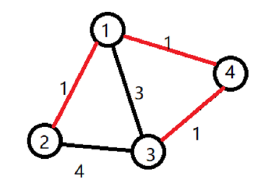
\includegraphics[width=5cm]{treasure_1.png}\end{center}
	小明选定让赞助商打通了 $1$ 号宝藏屋。小明开发了道路 $1 \to 2$,挖掘了 $2$ 号宝藏。开发了道路 $1 \to 4$,挖掘了 $4$ 号宝藏。还开发了道路 $4 \to 3$,挖掘了 $3$ 号宝藏。工程总代价为:$1 \times 1 + 1 \times 1 + 1 \times 2 = 4$
	\ \\
	\textbf{【样例解释$2$】}

	\begin{center}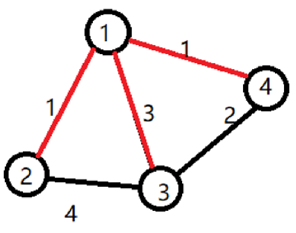
\includegraphics[width=5cm]{treasure_2.png}\end{center}

	小明选定让赞助商打通了 $1$ 号宝藏屋。小明开发了道路 $1 \to 2$,挖掘了 $2$ 号宝藏。开发了道路 $1 \to 3$,挖掘了 $3$ 号宝藏。还开发了道路 $1 \to 4$,挖掘了 $4$ 号宝藏。工程总代价为:$1 \times 1 + 3 \times 1 + 1 \times 1 = 5$
	\ \\
	\textbf{【数据规模与约定】}

	对于$20\%$的数据: 保证输入是一棵树,$1 \le n \le 8$,$v \le 5000$ 且所有的 v 都相等。

	对于$40\%$的数据: $1 \le n \le 8$,$0 \le m \le 1000$,$v \le 5000$ 且所有的 v 都相等。

	对于$70\%$的数据: $1 \le n \le 8$,$0 \le m \le 1000$,$v \le 5000$。

	对于$100\%$的数据: $1 \le n \le 12$,$0 \le m \le 1000$,$v \le 500000$。
\end{example}

一句话题意:
给定一个有重边,边有权值的无向图。从某一个点出发,求到达所有的点需要的最少费用,
并且限制两点之间只有一条路径。

费用的计算公式为:所有边的费用之和。而边(x\to y)的费用就为:y到初始点的距离 * 边权。

此题为NOIp 2017 Day2 T2。是一道比较基础的状压DP。有多种方法可以AC这道题目,正解有状压DP\sout{,模拟退火,遗传算法等等}。

会讲多种算法的。
\paragraph{随机化暴力}
dalao们应该都学习过搜索。搜索本质上就是个暴力。数据范围这么小,搜索是可以通过大部分数据的。是很划算的。

考虑随机一个点序列(在DFS时不按照输入顺序从1到n依次遍历整张图,容易被卡),然后指定一个定点为起点进行DFS计算出当前的花费(当然不一定要对整张图进行一次DFS,稍微剪一下枝),符合题意时更新一下答案就行了。当然这种算法在RP不好的时候会输出最大值,但这就是小概率事件了,况且可以多次对这个图进行随机化DFS。

考虑DFS的终止条件,由于我们希望图是一棵树(此时边数最小并且任意两点都可达),所以终止条件应该是找到了一棵树,即当前已经DFS过的点数等于$n+1$(联系最小生成树理解一下?)。

代码:
\begin{minted}{C++}
#include<cctype>
#include<cstdio>
#include<algorithm>
using namespace std;
#define N 20
#define fr(_a,_b,_c) for(int _a=_b;_a<=_c;_a++)
inline int read()
{
	char ch=getchar();int ret=0,flag=1;
	while(!isdigit(ch)&&ch!='-')ch=getchar();
	if(ch=='-')flag=-1;
	while(isdigit(ch))ret=ret*10+ch-'0',ch=getchar();
	return flag*ret;
}
int n,m,d[N][N],ans,t[N],h[N];
void dfs(int x,int w)//x表示当前DFS过的点的个数,w表示当前状态下的花费。
{
    if(ans<=w)//剪枝:如果已经找到的答案比当前状态下的花费小,回溯。
        return;
    if(x==n+1)//更新解,如果DFS到了一棵树并且需要更新答案,更新答案。
    {
        ans=w;
        return;
    }
    for(int i=1;i<=x-1;i++)
        if(d[t[x]][t[i]]+1)
        {
            h[t[x]]=h[t[i]]+1;
            dfs(x+1,w+d[t[x]][t[i]]*h[t[x]]);
        }
}
int main()
{
    n=read();
    m=read();
    fr(i,1,n)
        fr(j,1,n)
            d[i][j]=-1;
    fr(i,1,m)
    {
        int u=read(),v=read(),w=read();
        if(d[u][v]==-1)
            d[u][v]=d[v][u]=w;
        else
            d[u][v]=d[v][u]=min(d[u][v],w);
    }
    ans=(1<<20);
    fr(i,1,n)
        t[i]=i;
    srand((unsigned long long)new char);
    fr(i,1,5040)
    {
        fr(i,1,n*n)
            swap(t[rand()%n+1],t[rand()%n+1]);
        fr(i,1,n)
            h[i]=0;
        dfs(2,0);
    }
    printf("%d\n",ans);
    return 0;
}
\end{minted}

时间复杂度$O(5040\times 3^n)$,期望得分0~100.
\paragraph{模拟退火}
在介绍模拟退火算法之前先介绍一下TSP问题和TSP问题所属的NP问题和NPC问题。
\begin{definition}[NP问题] 是指存在多项式算法能够解决的非决定性问题,而其中NP完全问题又是最有可能不是P问题的问题类型。所有的NP问题都可以用多项式时间划归到他们中的一个。所以显然NP完全的问题具有如下性质:它可以在多项式时间内求解,当且仅当所有的其他的NP完全问题也可以在多项式时间内求解。
\end{definition}
以上是NP问题的定义,所谓多项式算法就是时间复杂度可以写作$O(n^a), $\\$a\in \mathbf{R}$的形式的算法。
\begin{definition}[NPC问题]NP中的某些问题的复杂性与整个类的复杂性相关联。这些问题中任何一个如果存在多项式时间的算法,那么所有NP问题都是多项式时间可解的。这些问题被称为NP完全问题(NPC问题)。
\end{definition}
	以上是对NPC问题的定义,换句话说就是不容易有有效算法的问题(需要搜索、枚举等等很暴力的算法来解决的问题)。
	\begin{definition}[TSP问题]又译为旅行推销员问题、货郎担问题,是数学领域中著名问题之一。问题的一般形式类似于“假设有一个旅行商人要拜访n个城市,他必须选择所要走的路径,路径的限制是每个城市只能拜访一次,而且最后要回到原来出发的城市。路径的选择目标是要求得的路径路程为所有路径之中的最小值。”

		\textbf{TSP问题可以被证明是一个NPC问题。}
	\end{definition}
	以上是对TSP问题的定义,要注意到这是一个NPC问题。
	\begin{definition}[模拟退火算法]是一种通用概率演算法,用来在一个大的搜寻空间内找寻命题的最优解。模拟退火算法是解决TSP(旅行商问题)的有效方法之一。

		模拟退火的出发点是基于物理中固体物质的退火过程与一般组合优化问题之间的相似性。模拟退火算法是一种通用的优化算法,其物理退火过程由加温过程、等温过程、冷却过程这三部分组成。
	\end{definition}
	可以看到,模拟退火是解决需要搜索的问题的一种有效算法(但是只针对于部分问题,不具有普适性)。

	转回来看这个题,由于答案具有比较强的连续性(可能与随机数据等等有关),所以模拟退火算法适用于这道题目。

	考虑下图所示的函数图像:
	\begin{center}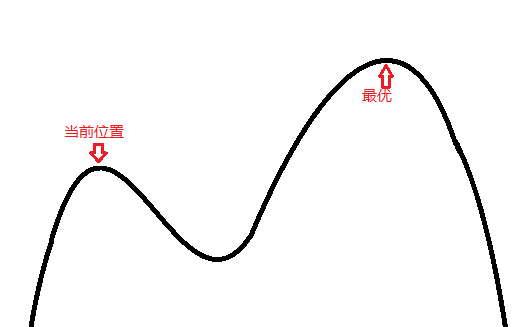
\includegraphics[scale=0.3]{sa.png}\end{center}
	如果坚决不接受较差的解,那么我们就无法到达最优解所在的位置。这使我们必须接受存在较差的解(但不能全部接受,否则就与搜索一样了)。我们可以写一个接受函数来决定是否接受这个解。假设答案越小越优,我们可以得到以下接受函数:
	\begin{minted}{C++}
bool accept(double delta, double temper)//delta表示函数的变化量,temper表示当前“温度”,“温度”随时间推移缓慢减小,从而实现“退火”的过程。
{
    if(delta <= 0) return true;//如果找到了更优的解,就接受。
    return rand() <= exp((-delta) / temper) * RAND_MAX;//随机接受较差的解。
}
\end{minted}
	下面解释一下第二行接受较差的解的代码:

	我们将$\textrm{rand()}\leq \exp(\frac{-\Delta}{temper})\times\textrm{RAND\_MAX}$移项,可得:
$\frac{\textrm{rand()}}{\textrm{RAND\_MAX}}\leq\exp(\frac{-\Delta}{temper})$,根据定义$temper$始终为正,而$\Delta$为正数,所以$\exp()$函数的自变量为负数。由指数函数的定义,返回值应该在区间(0,1)之间,定为接受的概率。而左边随机生成了一个实数,如果比概率小就接受,否则就不接受。

	简单来说,就是随机化接受较差的解,从而达到到达最优解的过程。由于“温度”随时间推移缓慢减小,所以跳往较差解的概率也下降。

	模拟退火的原理是,通过赋予搜索过程一种时变且最终趋于零的概率突跳性,从而可有效避免陷入局部极小并最终趋于全局最优的串行结构的优化算法。由于这个原理的限制,模拟退火算法能找到的最优解可能不是最优解,但是与最优解已经非常相近了。这个特性比较适合做较高水平的比赛中的提交答案题,可能能艹掉标程,获得更高的分数。但是对于传统型题目,就很有可能WA掉。

	结合这题的代码理解一下模拟退火的流程:
	\begin{minted}{C++}
#include<bits/stdc++.h>
using namespace std;
const int maxn=110;
const int maxm=2010;
int mp[maxn][maxn],n,m,i,j,k,x,y,z,ans,s;
int a[maxn],b[maxn],c[maxn],ha[maxn],oldf,newf,vis[maxn];
double T;//模拟退火中的温度
int read()
{
    int tot=0,fh=1;
    char c=getchar();
    while((c-'0'<0)||(c-'0'>9)){if(c=='-')fh=-1;c=getchar();}
    while((c-'0'>=0)&&(c-'0'<=9)){tot=tot*10+c-'0';c=getchar();}
    return tot*fh;
}
int dfs(int x,int dep)//遍历这张图,x表示当前点的编号,dep表示当前遍历过的点的个数
{
    if (dep>13) return 0;//如果已经不是一棵树了,不符合题中“小明不想开发无用道路,即两个已经被挖掘过的宝藏屋之间的道路无需再开发”这一条件,进行剪枝。
    if (x!=s){vis[x]=dfs(c[x],dep+1);return vis[x];}//若还未到达终点就继续进行DFS。
    else return 1;//若到达终点表示这是一组可行解。
}
int check()
{
    int i;
    memset(vis,0,sizeof(vis));
    for (i=1;i<=n;i++)//以每一个点为起点进行DFS
    {
        if (vis[i]==0) vis[i]=dfs(i,1);//vis[i]表示以i号点为起点是否存在可行解。
        if (vis[i]==0) return 0;//不存在可行解
    }
    return 1;
}
int dfs2(int x)//用于计算$\sum L_i\times K_i$新值的搜索,x表示当前点的编号。
{
    if ((s==x)||(vis[x]!=0)) return vis[x];//如果是起点或者已经被访问过了就返回x点的深度。
    int t1=dfs2(c[x])+1;//记录深度,即题目中的K
    vis[x]=t1;//记录当前点的深度
    newf=newf+t1*mp[c[x]][x];//更新$\sum L_i\times K_i$的值
    return t1;
}
void getnewf()//对dfs2()的封装,用于计算$\sum L_i\times K_i$的值
{
    int i;
    newf=0;
    memset(vis,0,sizeof(vis));
    for (i=1;i<=n;i++)//以每个点为起点进行DFS
    {
        if (vis[i]==0) dfs2(i);//如果没被访问过,即当前点对答案的贡献还没有计算进去,就计算一下从当前点可以增广到的点的距离。
    }
}
void bfs(int x)//寻找近似解
{
    int l=1,r=1,i; a[l]=x; oldf=0; b[x]=0;
    memset(ha,-1,sizeof(ha)); ha[x]=0;
    while (l<=r)
    {
        for (i=1;i<=n;i++)
        {
            if ((ha[i]==-1)&&(mp[a[l]][i]!=1e9))//如果没有被增广过并且l与i之间有边
            {
                ha[i]=ha[a[l]]+1;//记录一下深度
                r++; a[r]=i;//入队
                b[i]=a[l];//记录一下父亲节点
                oldf=oldf+mp[a[l]][i]*ha[i];//计算原有的f函数
            }
        }
        l++;//旧节点出队
    }
    ans=min(ans,oldf);//两者取一个较小值。
}
int main()
{
    n=read(); m=read();
    for (i=1;i<=n;i++)
    {
        for (j=1;j<=n;j++)
        {
            if (i==j) mp[i][j]=0;
            else mp[i][j]=1e9;
        }
    }
    for (i=1;i<=m;i++)
    {
        x=read(); y=read(); z=read();
        mp[x][y]=min(mp[x][y],z);
        mp[y][x]=min(mp[y][x],z);
    }
    ans=1e9;
    srand(19260817);
    for (i=1;i<=n;i++)
    {
        s=i; bfs(i);//以每个点为起点进行一次BFS计算深度。
        if (n<=2) continue;//如果只有两个点,就不需要退火。
        for (T=10000;T>=0.00001;T=T*0.9999)//模拟退火过程,T表示温度。
        {
            x=(rand()%(n-1))+1; if (x>=i) x++;//随机指定起点和终点。
            y=(rand()%(n-1))+1;
            if (y>=x) y++;
            if (mp[x][y]==1e9) continue;//不连通
            for (j=1;j<=n;j++) c[j]=b[j];//复制一下b数组
            c[x]=y;//起点的父亲节点是终点。
            if (check()==0) continue;//如果不存在可行解跳出循环
            getnewf();//计算新的代价
            if ((newf<=oldf)||( exp((oldf-newf)/T))>=((rand()%1000000)/1000000.0))//接受函数,解释见上。
            {
                ans=min(ans,newf);//更新一下答案
                for (j=1;j<=n;j++) b[j]=c[j];//复制一下c数组
                oldf=newf;//刚刚计算出的函数值变成旧的函数值
            }
        }
    }
    printf("%d\n",ans);
    return 0;
}
\end{minted}

	时间复杂度$O(207223n^3)$.
	\paragraph{最小生成树}
	这是考场上很多人想到的非完美解法,当时在考场上好像是可以过1号样例,但是2号样例过不了。我在考场上也想到了这种方法,然而并没有写完,所以gg。

	考虑一下最小生成树的问题所在。Kruskal算法需要贪心地选择边权较小的边,所以如果枚举的点不在最小生成树上,贪心的结果就是错误的。

	就是说,如果到某一个点的最优路径不在最小生成树上(因为不仅仅是最小生成树上的点,如果一条边在最小生成树上,但是他的深度非常深,那么它对答案的贡献,即L\times K就会非常大),答案就不对了。有一组数据可以卡掉Prim算法(当然据说Prim可以过大数据,yyf dalao写过Kruskal好像是没有分)。

	至于卡掉最小生成树的数据的话,rqy dalao出了一组:
	\begin{minted}{text}
7 7
1 2 5000
2 3 1
3 4 1
4 5 1
5 6 2
2 7 9
6 7 3 
\end{minted}
	\paragraph{状压DP}
	考虑一个事实,给定一个加点序列,上一节提出的贪心的策略就是正确的了(计算答案的过程转化成类似最短路的东西)。

	所以枚举一下1~12的全排列,get到加点的序列,然后贪心就行了。

	但是这样时间复杂度就是$O(n!2^n)$,只能过一部分数据(可以拿到80分)。

	考虑题目要求构造一棵生成树,使得所有边的费用之和最小。问题转换为树上问题。

	设所有的点构成全集$U$,定义状态$f_{i,j}$表示考虑到树的第$i$层,前$i$层已选的点的集合为$S$(使用二进制压缩状态)的最小代价。

	状态的转移可以枚举所有不在S中的集合(令集合$S'\subseteq(\complement_U S)$,枚举集合$S'$)作为树的第$i+1$层。

	状态转移:
	\begin{equation*}
		dp[i][S]\to dp[i+1][S|S']+(i+1)\times shortestPath[S'][S]
	\end{equation*}

	其中$shortestPath[S'][S]$表示从集合$S'$到集合$S$的最短距离(需要提前用Floyd算法预处理两点间的最短路,然后处理出来),如果理解不了就看一下上面对集合间最短距离的定义,就是枚举集合$S$与集合$S'$所有点对(a,b)所在集合$P=\{p(a,b)\mid a\in S, b\in S', S\cap S'=\emptyset\}$,点对$p(a,b)$的最短路长度之和,程序中使用$pval$数组保存了每个点对之间的最短路,然后再转化成集合之间的距离,存储到$sval$数组里面。

	DP的顺序:由DP方程,由大到小枚举层数,然后枚举集合就行了。

	边界条件:枚举根节点,则$dp[0][1\text{<\!<}(root-1)]=0$。

	代码:
	\begin{minted}{C++}
#include<cstdio>
#include<algorithm>
using namespace std;
typedef long long LL;
const int INF = 1e7;
const int N = 13;
int n, m, g[N][N], u, v, p, U;
LL dp[N][1<<N], ans = 1e14, sval[1<<N][1<<N], pval[N][1<<N];
void init(int root)//初始化DP数组,建树,将边界条件设置好 
{
    for(int i = 0; i <= n; i++)
        for(int j = 0; j <= U; j++)
            dp[i][j] = INF;
    dp[0][1<<(root-1)] = 0;
}
int main()
{
    scanf("%d%d", &n, &m);
    U = (1 << n) - 1;
    for(int i = 1; i <= n; i++)//初始化图、DP数组、最短路数组 
        for(int j = 1; j <= n; j++)
            if(i ^ j)
                g[i][j] = INF;
    for(int i = 1; i <= n; i++)
        for(int j = 0; j <= U; j++)
            pval[i][j] = INF;
    for(int i = 0; i <= U; i++)
        for(int j = 0; j <= U; j++)
            sval[i][j] = INF;
    while(m--)//邻接矩阵加边,注意有重边的情况取较小值。 
    {
        scanf("%d%d%d", &u, &v, &p);
        g[u][v] = min(g[u][v], p);
        g[v][u] = min(g[v][u], p);
    }
    for(int i = 1; i <= n; i++)//预处理所有满足条件的点对(a,b)之间的最短路,使用Floyd算法 
        for(int j = 0; j <= U; j++)
            for(int k = 1; k <= n; k++)
                if(j & (1 << (k - 1)))
                    pval[i][j] = min(pval[i][j], 1ll*g[i][k]);
    for(int i = 0; i <= U; i++)//预处理集合之间的距离 
    {
        int C = i ^ U;//求出$\complement_U S$
        for(int s = C; s; s = (s - 1) & C)
        {
            LL temp = 0;
            for(int j = 1; j <= n; j++)
                if(s & (1 << (j - 1)))
                    temp += pval[j][i];
            sval[s][i] = temp >= INF ? INF : temp;
        }
    }
    for(int root = 1; root <= n; root++)//枚举每一个根 
    {
        init(root);
        for(int i = 0; i < n; i++)//枚举每一个点 
            for(int S = 0; S <= U; S++)//枚举每一个集合 
                if(dp[i][S] != INF)
                {
                    int C = S ^ U;//求出$\complement_U S$ 
                    for(int s = C; s; s = (s - 1) & C)
                        dp[i+1][S|s] = min(dp[i+1][S|s], dp[i][S] + (i + 1) * sval[s][S]);//这里的'|'运算符是对集合做的运算,相当于求集合的并。 
                }
        for(int i = 0; i < n; i++)  ans = min(ans, dp[i][U]);
    }
    printf("%lld", ans);
    return 0;
}
\end{minted}

	时间复杂度$O(n^2\times 2^n)=84934656<10^8$,可以通过所有数据。

	这样的话,状压DP就讲完了。还是有些难理解的,我讲的可能不是很清楚,课下好好理解一下吧。

	(其实状压DP一般可以用启发式搜索或者是记忆化搜索水过去,就像前面讲的随机化暴力和模拟退火算法一样)
	\note
	\subsection{数位DP}
	\subsubsection{基础知识}
	\begin{definition}[数位DP]数位dp是一种计数用的dp,一般就是要统计一个区间$[le,ri]$内满足一些条件数的个数。
	\end{definition}
	以上是对于数位DP的定义。

	做关于数位的题目首先考虑一下枚举方式:
	\begin{enumerate}
		\item{\begin{minted}{C++}
for(int i=le;i<=ri;i++)  
    if(right(i)) ans++;
\end{minted}
		      无法记忆化搜索。gg。}
		\item{控制上界,按位从高到低枚举。
		      注意枚举时从高位开始,前导零也要枚举。
		      需要注意的是枚举是从``00001"这样开始枚举,一直枚举到小于右边界。}
	\end{enumerate}
	
	基本的动态模板:
	\begin{minted}{C++}
typedef long long ll;  
int a[20];  
ll dp[20][state];//不同题目状态不同  
ll dfs(int pos,/*state变量*/,bool lead/*前导零*/,bool limit/*数位上界变量*/)//不是每个题都要判断前导零  
{  
    //递归边界,既然是按位枚举,最低位是0,那么pos==-1说明这个数我枚举完了  
    if(pos==-1) return 1;/*这里一般返回1,表示你枚举的这个数是合法的,那么这里就需要你在枚举时必须每一位都要满足题目条件,也就是说当前枚举到pos位,一定要保证前面已经枚举的数位是合法的。不过具体题目不同或者写法不同的话不一定要返回1 */  
    //第二个就是记忆化(在此前可能不同题目还能有一些剪枝)  
    if(!limit && !lead && dp[pos][state]!=-1) return dp[pos][state];  
    /*常规写法都是在没有限制的条件记忆化,这里与下面记录状态是对应,具体为什么是有条件的记忆化后面会讲*/  
    int up=limit?a[pos]:9;//根据limit判断枚举的上界up;这个的例子前面用213讲过了  
    ll ans=0;  
    //开始计数  
    for(int i=0;i<=up;i++)//枚举,然后把不同情况的个数加到ans就可以了  
    {  
        if(...)
        else if(...)  
        ans+=dfs(pos-1,/*状态转移*/,lead && i==0,limit && i==a[pos]) //最后两个变量传参都是这样写的  
        /*这里还算比较灵活,不过做几个题就觉得这里也是套路了 
        大概就是说,我当前数位枚举的数是i,然后根据题目的约束条件分类讨论 
        去计算不同情况下的个数,还有要根据state变量来保证i的合法性,比如题目 
        要求数位上不能有62连续出现,那么就是state就是要保存前一位pre,然后分类, 
        前一位如果是6那么这意味就不能是2,这里一定要保存枚举的这个数是合法*/  
    }  
    //计算完,记录状态  
    if(!limit && !lead) dp[pos][state]=ans;  
    /*这里对应上面的记忆化,在一定条件下时记录,保证一致性,当然如果约束条件不需要考虑lead,这里就是lead就完全不用考虑了*/  
    return ans;  
}  
ll solve(ll x)  
{  
    int pos=0;  
    while(x)//把数位都分解出来  
    {  
        a[pos++]=x%10;//个人老是喜欢编号为[0,pos),看不惯的就按自己习惯来,反正注意数位边界就行  
        x/=10;  
    }  
    return dfs(pos-1/*从最高位开始枚举*/,/*一系列状态 */,true,true);//刚开始最高位都是有限制并且有前导零的,显然比最高位还要高的一位视为0嘛  
}  
int main()  
{  
    ll le,ri;  
    while(~scanf("%lld%lld",&le,&ri))  
    {  
        //初始化dp数组为-1,这里还有更加优美的优化,后面讲  
        printf("%lld\n",solve(ri)-solve(le-1));  
    }  
}  
\end{minted}

	为了做到无遗漏的枚举,代码中的limit变量就是用于判断枚举位置。
	最重要的问题在于“枚举上界”。如果不能理解的话,举个例子:
	枚举上界为219。
	假设已经枚举最高位为1,因为$0\le 2$,所以十位上怎么枚举也不会超过上界,limit应该为false,表示对这一位的枚举没有上界限制;
	假设枚举最高位为2,此时对十位的枚举就应该有限制,枚举上界为1;
	(对高位的枚举对低位有影响。)
	当然对位数小于ri的数来说,怎么枚举也没有问题,需要枚举上。
	想想判limit与不判limit记忆化搜索的不同。
	假设没判limit,那么假设我们第一次枚举了百位是0,显然后面的枚举limit=false,也就是数位上0到9的枚举,然后当我十位枚举了1,此时考虑dp[0][1],就是枚举到个位,前一位是1的个数,显然dp[0][1]=9;(个位只有是1的时候是不满足的),这个状态记录下来,继续dfs,一直到百位枚举了2,十位枚举了1,显然此时递归到了pos=0,pre=1的层,而dp[0][1]的状态已经有了即dp[pos][pre]!=-1;此时程序直接return dp[0][1]了,然而显然是错的,因为此时是有limit的个位只能枚举0,根本没有9个数,这就是状态冲突了。有lead的时候可能出现冲突,这只是两个最基本的不同的题目可能还要加限制,反正宗旨都是让dp状态唯一。
	有两点需要说明:
	\begin{enumerate}
		\item{limit为true的情况并不会非常多,逐个进行判断也不会特别浪费时间,所以需要记录一下,以解决子问题重叠的问题。}
		\item{DP状态可以改为dp[pos][status][limit],给limit也记忆化,记录不同的limit的个数,这种方法一般是对的。有些题目需要这样优化。}
	\end{enumerate}
	还涉及另一个问题。因为仅仅限制了枚举的上界,求出来的值不一定是原来题目要求的区间内的答案(实际上是区间[0,ri]的答案),所以要对答案进行一些处理。
	\begin{minted}{C++}
int main()  
{  
    long long le,ri;  
    while(~scanf("%lld%lld",&le,&ri))  
        printf("%lld\n",solve(ri)-solve(le-1));  
}  
\end{minted}

	上面的代码事实上就是对区间[0,ri]与[li,ri]取一个交集的过程,由高中数学的集合运算法则$A\cap B=A(A\subseteq B)$而来。

	DP的话,同记忆化搜索。状态一般是与前面已经枚举的数位有关,并且往往是对连续$k$位有要求,就保存前面$k-1$位的状态,然后当前枚举第$k$位,和前$k-1$位恰好拼凑出完整的状态。当然如果状态是数位的和,就直接保存数位的前缀和。
	\subsubsection{入门例题---不要62}
	我们来看一道入门难度的例题。
	\begin{example}
		HDU2089 不要62\\
		\textbf{题目描述}

		杭州人称那些傻乎乎粘嗒嗒的人为62(音:laoer)。

		杭州交通管理局经常会扩充一些的士车牌照,新近出来一个好消息,以后上牌照,不再含有不吉利的数字了,这样一来,就可以消除个别的士司机和乘客的心理障碍,更安全地服务大众。

		不吉利的数字为所有含有4或62的号码。例如:\verb+62315 73418 88914+都属于不吉利号码。但是,61152虽然含有6和2,但不是62连号,所以不属于不吉利数字之列。

		你的任务是,对于每次给出的一个牌照区间号,推断出交管局今次又要实际上给多少辆新的士车上牌照了。\\
		\textbf{输入格式}

		输入的都是整数对n、m($0\leq n\leq m\leq 1000000$),如果遇到都是0的整数对,则输入结束。\\
		\textbf{输出格式}

		对于每个整数对,输出一个不含有不吉利数字的统计个数,该数值占一行位置。\\
		\textbf{样例输入}
		\begin{minted}{text}
1 100
0 0
\end{minted}
		\textbf{样例输出}
		\begin{minted}{text}
80
\end{minted}
	\end{example}

	就是数位上不能有4也不能有连续的62,没有4的话在枚举的时候判断一下,不枚举4就可以保证状态合法了,所以这个约束没有记忆化的必要,而对于62的话,涉及到两位,当前一位是6或者不是6这两种不同情况我计数是不相同的,所以要用状态来记录不同的方案数。

	dp[pos][sta]表示当前第pos位,前一位是否是6的状态,这里sta只需要去0和1两种状态就可以了,不是6的情况可视为同种,不会影响计数。
	
	代码:
	\begin{minted}{C++}
#include<iostream>  
#include<cstdio>  
#include<cstring>  
#include<string>  
using namespace std;  
typedef long long ll;  
int a[20];  
int dp[20][2];  
int dfs(int pos,int pre,int sta,bool limit)  
{  
    if(pos==-1) return 1;  
    if(!limit && dp[pos][sta]!=-1) return dp[pos][sta];  
    int up=limit ? a[pos] : 9;  
    int tmp=0;  
    for(int i=0;i<=up;i++)  
    {  
        if(pre==6 && i==2)continue;  
        if(i==4) continue;//都是保证枚举合法性  
        tmp+=dfs(pos-1,i,i==6,limit && i==a[pos]);  
    }  
    if(!limit) dp[pos][sta]=tmp;  
    return tmp;  
}  
int solve(int x)  
{  
    int pos=0;  
    while(x)  
    {  
        a[pos++]=x%10;  
        x/=10;  
    }  
    return dfs(pos-1,-1,0,true);  
}  
int main()  
{  
    int le,ri;  
    //memset(dp,-1,sizeof dp);可优化  
    while(~scanf("%d%d",&le,&ri) && le+ri)  
    {  
        memset(dp,-1,sizeof dp);  
        printf("%d\n",solve(ri)-solve(le-1));  
    }  
    return 0;  
}  
\end{minted}

	\sout{其实还是记忆化搜索。}
	\subsubsection{常数优化}
	讲一个常数优化,放在ACM赛制中比较好用。

	把memset放在多组数据以外。由于数位DP的特点,DP状态与数本身有关,而不是与数据的组数有关,所以之前的状态还可以继续使用。

	求数位和是10的倍数的个数,这里简化为数位sum\%10这个状态,即dp[pos][sum]这里10是与多组无关的,所以可以memset优化,不过注意如果题目的模数是输入的话那就不能这样了。
	\subsubsection{减法的艺术---F(x)}
	先来看一道例题。
	\begin{example} HDU4734 F(x)\\
	\textbf{题目描述}
	
	对于一个有$n$位的十进制数$x(A_nA_{n-1}A_{n-2}\cdots A_2A_1)$,我们定义它的权值为:
	\begin{equation*}
	F(x)=A_n\times 2^{n-1}+A_{n-1}\times 2^{n-1}+A_{n-2}\times 2^{n-2}+\cdots+A_2\times 2+A_1\times 1.
	\end{equation*}
	
给定两个数A和B,请计算在区间$[0,B]$内有多少个数权值不超过F(A)。\\
	\textbf{输入格式}
	
	第一行包含一个数$T(T\leq 10000)$,表示测试数据组数;
	
	对于每一组测试数据,都有两个数$A$和$B(0\leq A, B\leq 10^9)$。\\
	\textbf{输出格式}
	
	对于每一组数据,你应该先输出`` \verb+Case #t: + ''(不包含引号),$t$是测试数据编号,从$1$开始。然后输出答案。\\
	\textbf{样例输入}
\begin{minted}{text}
3
0 100
1 10
5 100
\end{minted}
\textbf{样例输出}
\begin{minted}{text}
Case #1: 1
Case #2: 2
Case #3: 13
\end{minted}
	\end{example}

常规想:这个f(x)计算就和数位计算是一样的,就是加了权值,所以dp[pos][sum],这状态是基本的。a是题目给定的,f(a)是变化的不过f(a)最大好像是4600的样子。如果要memset优化就要加一维存f(a)的不同取值,那就是dp[10][4600][4600],这显然不合法。

这个时候就要用减法了,dp[pos][sum],sum不是存当前枚举的数的前缀和(加权的),而是枚举到当前pos位,后面还需要凑sum的权值和的个数,也就是说初始的是时候sum是f(a),枚举一位就减去这一位在计算f(i)的权值,那么最后枚举完所有位 sum\leq 0时就是满足的,后面的位数凑足sum位就可以了。

仔细想想这个状态是与f(a)无关的,一个状态只有在sum\leq 0时才满足,如果我们按常规的思想求f(i)的话,那么最后sum\leq f(a)才是满足的条件。

这道题目展示了前缀和在数位DP中的重要作用。希望大家理解一下。以下是代码:
\begin{minted}{C++}
#include<cstdio>  
#include<cstring>  
#include<iostream>  
#include<string>  
  
using namespace std;  
const int N=1e4+5;  
int dp[12][N];  
int f(int x)  
{  
    if(x==0) return 0;  
    int ans=f(x/10);  
    return ans*2+(x%10);  
}  
int all;  
int a[12];  
int dfs(int pos,int sum,bool limit)  
{  
    if(pos==-1) {return sum<=all;}  
    if(sum>all) return 0;  
    if(!limit && dp[pos][all-sum]!=-1) return dp[pos][all-sum];  
    int up=limit ? a[pos] : 9;  
    int ans=0;  
    for(int i=0;i<=up;i++)  
    {  
        ans+=dfs(pos-1,sum+i*(1<<pos),limit && i==a[pos]);  
    }  
    if(!limit) dp[pos][all-sum]=ans;  
    return ans;  
}  
int solve(int x)  
{  
    int pos=0;  
    while(x)  
    {  
        a[pos++]=x%10;  
        x/=10;  
    }  
    return dfs(pos-1,0,true);  
}  
int main()  
{  
    int a,ri;  
    int T;  
    int kase=1;  
    scanf("%d",&T);  
    memset(dp,-1,sizeof dp);  
    while(T--)  
    {  
        scanf("%d%d",&a,&ri);  
        all=f(a);  
        printf("Case #%d: %d\n",kase++,solve(ri));  
    }  
    return 0;  
}  
\end{minted}
	\note